% Kelompok Diagram Kartesius
% Rahmi Nurdin (1154109)
% Mustari Muammar (1154108)
% Fadillah Firdaus (1154103)

\section{Pengertian Diagram Kartesius}
Diagram Kartesius adalah sistem kooordinat yang terdiri dari dua sumbu yang berisi titik-titik sebagai simbol relasi.
Domain sebagai sumbu horizontal dan kodomain sebagai sumbu vertikal.
Pada koordinat kartesius daerah asal (domain) diletakkan pada sumbu X (sumbu mendatar) dan daerah kawan (kodomain) diletakkan pada sumbu Y (sumbu tegak).
Sedangkan daerah hasilnya merupakan titik (noktah) koordinat pada diagram kartesius. Dari relasi di atas, dapat ditunjukkan diagram kartesiusnya seperti di bawah :
\begin{figure}[ht]
	\centerline{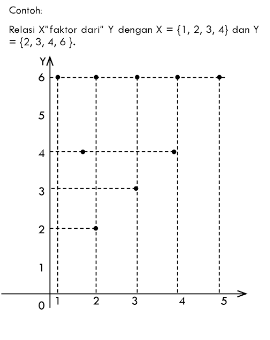
\includegraphics[width=1\textwidth]{figures/rahmi1.PNG}}
	\caption{hubungan antar titik pada diagram kartesius.}
	\label{rahmi1}
	\end{figure}

Diagram Kartesius merupakan suatu bangunan atas empat bagian yang batasi oleh dua buah garis yang berpotongan tegak lurus pada titik-titik (  X, Y ). 
Dimana X merupakan rata-rata dari rata-rata skor tingkat pelaksanaan atau kepuasan konsumen dari sebuah faktor atribut 
dan Y adalah rata-rata skor tingkat kepentingan seluruh faktor atau atribut yang mempengaruhi kepuasan konsumen.
Seluruhnya ada K faktor. Rumus berikutnya yang digunakan adalah :
\begin{figure}[ht]
	\centerline{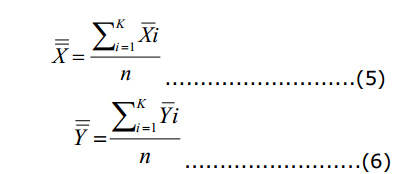
\includegraphics[width=1\textwidth]{figures/rahmi2.PNG}}
	\caption{rumus mencari K faktor.}
	\label{rahmi2}
	\end{figure}

Dimana :K = Banyaknya faktor atau atribut yang mempengaruhi kepuasan konsumen 
Diagram Kartesius	
\begin{figure}[ht]
	\centerline{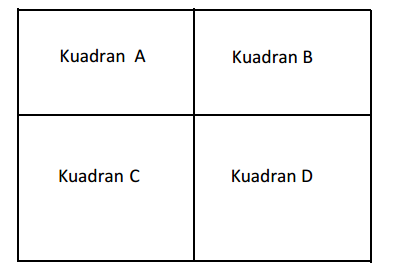
\includegraphics[width=1\textwidth]{figures/rahmi3.PNG}}
	\caption{penentuan kuadran pada diagram kartesius.}
	\label{rahmi3}
	\end{figure}

Gambar 1. Diagram Kartesius



Kuadran A
Pada posisi ini, jika dilihat dari kepentingan konsumen, atribut-atibut produk berada pada tingkat tinggi, tetapi jika di lihat dari kepuasannya, 
konsumen merasakan tingkat yang rendah, sehingga konsumen menuntut adanya perbaikan atribut tersebut.
Kuadran B
Pada posisi ini, jika dilihat dari kepentingan konsumen, atribut-atribut produk berada pada tingkat tinggi, dan dilihat dari kepuasannya, 
konsumen merasakan tingkat yang tinggi juga.
Kuadran C
Pada posisi ini, jika dilihat dari kepentingan konsumen, atribut-atribut produk kurang dianggap penting, tetapi jika dilihat dari tingkat kepuasan konsumen cukup baik.
Namun, konsumen mengabaikan atributatribut yang terletak pada posisi ini.
Kuadran D
Pada posisi ini, jika dilihat dari kepentingan konsumen, atribut-atribut produk kurang dianggap penting, tetapi jika dilihat dari tingkat kepuasanya, konsumen merasa
sangat puas.


\section{Penghitungan Rumus Diagram Kartesius}
\subsection{meghitung rumus, mencari titik}

Kartesius digunakan untuk menentukan tiap titik dalam bidang dengan menggunakan dua bilangan yang biasa disebut koordinat x dan koordinat y.
\begin{figure}[ht]
	\centerline{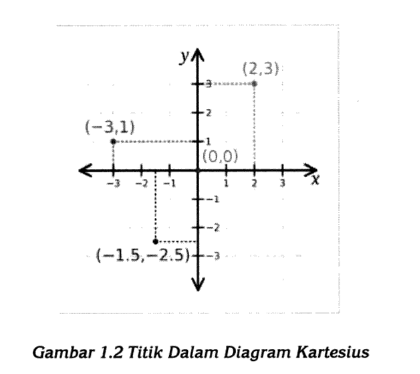
\includegraphics[width=1\textwidth]{figures/rahmi9.PNG}}
	\caption{penentuan titik pada kuadran katesius.}
	\label{rahmi9}
	\end{figure}

Sebuah titik dalam Diagram Kartesius, mengandung dua buah informasi yakni sumbu (x,y), seperti tampak pada Gambar 1.2. 
Yaitu titik (2,3) adalah titik dimana nilai x=2 dan y=3. Daerah ini dikenal dengan kuadran I, dimana nilai x dan y adalah positif.
\begin{figure}[ht]
	\centerline{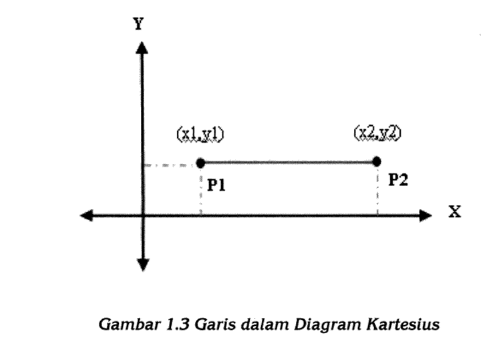
\includegraphics[width=1\textwidth]{figures/rahmi10.PNG}}
	\caption{penentuan garis pada kuadran katesius.}
	\label{rahmi10}
	\end{figure}

Dari dua buah titik diagram kartesius, bisa ditarik menjadi sebuah garis. Artinya pada sebuah garis memiliki titik awal


\section{Contoh Penerapan/Pemetaan Diagram Kartesius}
Tujuan digunakannya diagram kartesius adalah untuk melihat secara lebih terperinci mengenai atribut-atribut yang perlu untuk dilakukan perbaikan. 
Langkahlangkah sebelum memetakan data ke diagram kartesius ini, adalah terlebih dahulu dengan menentukan nilai rata-ratasetiap atribut yaitu X dan Y, 
dimana nilai perhitungannya telah kita peroleh dari perhitung yang dilakukan sebelumnya.
Adapun hasil pembagian setiap atribut pada setiap kuadaran ditampilkan pada gambar 2
\begin{figure}[ht]
	\centerline{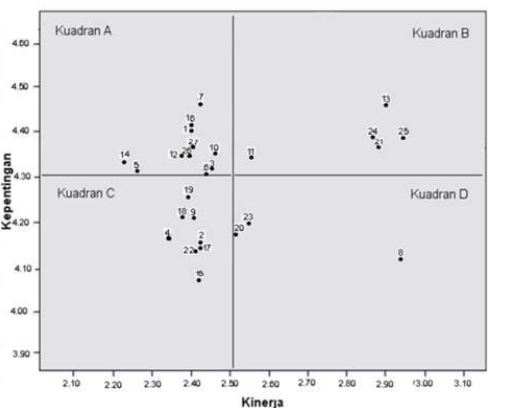
\includegraphics[width=1\textwidth]{figures/rahmi4.PNG}}
	\caption{.}
	\label{rahmi4}
	\end{figure}


Gambar 2. Diagram Kartesius
Setelah dilakukan perhitungan menggunakan diagram kartesius didapat hasil atribut-atribut yang harus diperbaiki adalah atribut yang berada pada kuadran A.
Adapun atribut yang harus diperbaiki pada kuadran A adalah :
Tabel 2 Hasil Perhitungan Diagram Kartesius pada Kuadran A	
\begin{figure}[ht]
	\centerline{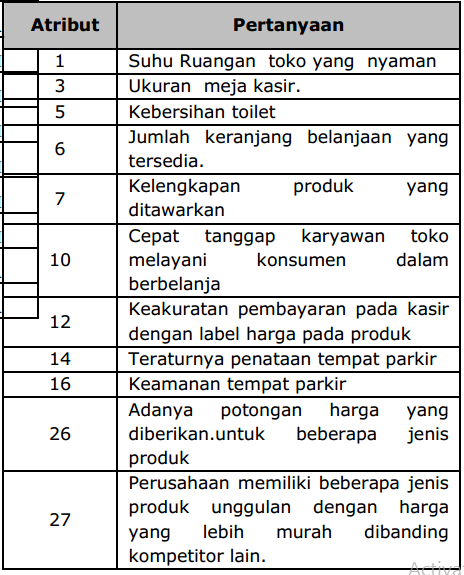
\includegraphics[width=1\textwidth]{figures/rahmi5.PNG}}
	\caption{.}
	\label{rahmi5}
	\end{figure}


Untuk atribut-atribut yang harus dipertahanan oleh pihak perusahaan setelah dilakukannya perhitungan menggunakan diagram kartesius adalah atribut-atribut
yang berada pada kuadran B, karena pada atribut yang berada pada kuadran B dianggap pelanggan sudah dapat memenuhi apa yang mereka inginkan. 
Adapun atribut yang harus dipertahankan dapat dilihat pada
Tabel 3.
Tabel 3. Hasil Perhitungan Diagram Kartesius
pada Kuadran B
\begin{figure}[ht]
	\centerline{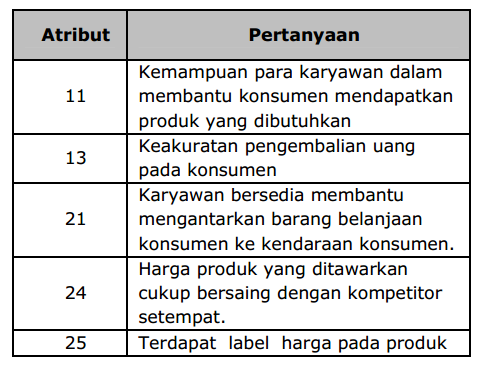
\includegraphics[width=1\textwidth]{figures/rahmi6.PNG}}
	\caption{.}
	\label{rahmi6}
	\end{figure}

Atribut yang memiliki penilaian yang rendah karena atribut-atribut ini kurang dianggap penting oleh pelanggan dan perusahaan juga tidak memberikan pelayanan atau perhatian khusus, 
atribut ini dianggap tidak memberikan dampak yang besar bagi perusahaan.
Adapun atribut-atribut yang berada pada kuadran C dapat dilihat pada Tabel 4.
Tabel 4. Hasil Perhitungan Diagram Kartesius pada kuadran C
\begin{figure}[ht]
	\centerline{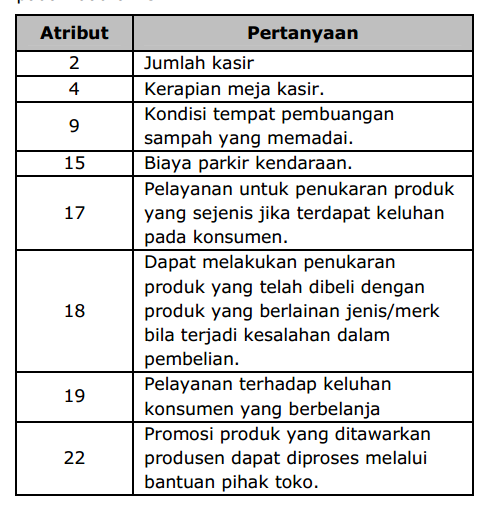
\includegraphics[width=1\textwidth]{figures/rahmi7.PNG}}
	\caption{.}
	\label{rahmi7}
	\end{figure}

Untuk atribut yang ada pada kuadran D adalah atribut yang tidak dianggap penting bagi pelanggan, namun pihak perusahaan memberikan pelayanan yang berlebihan 
sehingga atribut ini dianggap berlebihan.
Adapun atribut yang berada pada kuadran D dapat dilihat pada Tabel 5.
Tabel 5. Hasil Perhitungan Diagram Kartesius
pada Kuadran D	
\begin{figure}[ht]
	\centerline{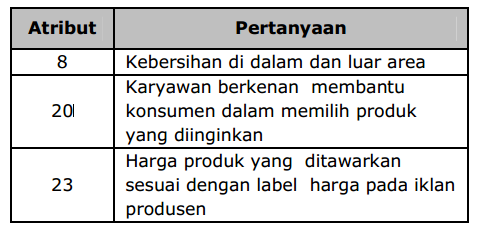
\includegraphics[width=1\textwidth]{figures/rahmi8.PNG}}
	\caption{.}
	\label{rahmi8}
	\end{figure}


Diagram Kartesius
Dari hasil perhitungan yang telah dilakukan sebelumnya, terdapat 17 atribut yang perlu dilakukan perbaikan (Action) danterdapat 10 atribut yang perlu mendapat
perhatian untuk dipertahankan oleh pihak perusahaan (Hold). Diagram Kartesius Dari hasil pemetaan yang dilakukan pada diagram kartesius dapat terlihat beberapa
atribut yang perlu untuk dilakukannya perbaikan dan atribut-atribut perlu untuk dipertahankan oleh pihak perusahaan yang terbagi kedalam kuadran-kuadran (A, B, C
dan D) sesuai dengan tingkat kesesuaian antara tingkat kepentingan pelanggan dan kinerja perusahaan, yaitu dengan tingkat kesesuaian sebesar 58.374.
Adapun hasil pemetaannya adalah sebagai berikut:
Kuadran A
Kuadran A adalah wilayah yang berisikan atribut-atribut yang dianggap penting oleh pelanggan, namun dalam kenyataannya atribut-atribut ini masih belum sesuai
dengan yang diharapkan oleh pelanggan. Dalam hal ini perusahaan perlu melakukan perbaikan sebaik mungkin untuk meningkatkan kepuasan pelanggan terhadap
atribut yang termasuk kedalam kuadran A. Dari diagram kartesius yang dibuat, diketahui bahwa atribut yang termasuk dalam kuadran A yaitu atribut 1, 3, 5, 6, 7,
10, 12, 14, 16, 26, 27.
Adapun beberapa hal yang sebaiknya perlu dilakukan guna perbaikan atau penyesuaian terhadap beberapa hal yang menjadi  prioritas diatas yang pertama antara lain
perlunya dilakukan penambahan alat pendingin ruangan untuk dapat menjaga suhu ruangan demi kenyamanan pelanggan,Penambahan ukuran meja kasir agarbarang-barang belanjaan yang telah dipilih
tidak merepotkan pelanggan ataupun kasir. Selain itu juga perlu dilakukannya perbaikan ataupun pembersihan ruangan toilet dan pendukung lainnya seperti ketersediaan air
sehingga pelanggan yang menggunakan akan merasa lebih nyaman, penambahan jumlah keranjang belanjaan yang disediakan perusahaan, Lebih melengkapi jenis-jenis
produk yang ditawarkan dengan mempertimbangkan tempat penyimpanan serta waktu-waktu tertentu seperti hari-hari besar nasional dan lain sebagainya,Memberikan pengarahan kepada para
karyawan mengenai pentingnya berinisiatif dalam melayani pelanggan yang membutuhkan bantuan tanpa harus dimintaitolong terlebih dahulu oleh pelanggan.
Dapat juga dilakukan penambahan papan informasi berupa lokasi produk yang tersedia untuk dapat mengurangi frekuensi terjadi atau timbulnya pertanyaan dari para
pelanggan mengenai produk yang akan mereka beli, perbaikan ataupun penyesuaian secara berkala antara labellabel harga yang tertera pada produk yang ditawarkan dengan perubahan-perubahan
harga yang terjadi, penataan tempat parkir yang dapat dilakukan dengan memberikan garis-garis pembatas kendaraan, ataupun dengan menambahkan tukang parkir untuk
dapat menanggulangi keamanan dan penataan tempat parkir kendaraan, penyusunan program-program promo secara berkala, seperti pemberian diskon denganjumlah pembelian tertentu ataupun dengan
memberikan voucer belanja dengan nilai tertentu untuk dapat lebih menarik pelanggan, dan sebaiknya perusahaan memiliki atau beberapa jenis produk tertentu
yang diunggulkan dengan harga yang lebih murah dibandingkan dengan kompetitor lainnya sebagai penarik.
Kuadran B
Kuadran B adalah daerah yang memuat atribut-atribut yang dianggap penting oleh pelanggan, dan atribut-atribut tersebut dianggap telah sesuai dengan keinginan
pelanggan sehingga tingkat kepuasan pelanggan relatif lebih tinggi, sehingga perlu untuk dipertahankan oleh pihak perusahaankarena sudah bisa memberikan pelayanan
sesuai dengan keinginan pelanggan sehingga konsumen merasa puas. Adapun atribut yang termasuk kedalam kuadran ini adalah:11, 13, 21, 24, 25.
Kuadran C
Kuadran C adalah Daerah yang berisikan atribut-atribut yang dianggap kurang penting oleh pelanggan dan pada kenyataannya kinerja pihak perusahaanpundinilai kurang memuaskan. Tetapi tidak
menutup kemungkinan Kuadran C pada waktu yang akan datang menjadi perhatian yang penting oleh pelanggan, sehingga perusahaan juga harus mempertimbangkan
hal tersebut. Adapun atribut yang termasuk kedalam kuadran ini adalah: 2, 4, 9, 15, 17, 18, 19, 22.
Kuadran D
Kuadran D adalah wilayah yang memuat atribut-atribut yang dianggap kurang penting oleh pelanggan dan kinerja yang dilakukan oleh pihak perusahaan dirasakan
terlalu tinggi atau berlebihan, sehingga perusahaan tidak perlu melakukan perbaikan. Adapun atribut yang termasuk kedalam kuadran ini adalah: 8, 20, 23.

\section{Pengertian Bidang atau Diagram Cartesius}

Dalam mempelajari materi himpunan, fungsi, dan persamaan garis lurus kita akan mengenal yang namanya bidang atau diagram Cartesius. Apa itu bidang atau diagram Cartesius?

Diagram Cartesius adalah sistem kordinat yang digunakan untuk meletakan titik pada penggambaran objek berdasarkan pemasukan nilai pada sumbu x dan nilai pada sumbu y dimana titik pertemuan ini nilai dari sumbu x dan sumbu y titik kordinat dibentuk. Jadi, diagram Cartesius digunakan untuk menentukan tiap titik dalam bidang dengan menggunakan dua bilangan yang biasa disebut koordinat x dan koordinat y dari titik tersebut. Di mana x disebut absis dan y disebut ordinat.

Titik-titik pada koordinat Cartesius merupakan pasangan titik pada sumbu-x dan sumbu-y (x, y). Perpotongan antara sumbu-x dan sumbu-y di titik 0 (nol) disebut pusat koordinat. Untuk bagian atas sumbu y bernilai positif, sedangkan pada bagian bawah sumbu y bernilai negatif. Begitu juga pada sebelah kanan sumbu x bernilai positif, sedangkan pada sebelah kiri sumbu x bernilai negatif. Untuk contohnya silahkan lihat gambar di bawah ini. 
\begin{figure}[ht]
	\centerline{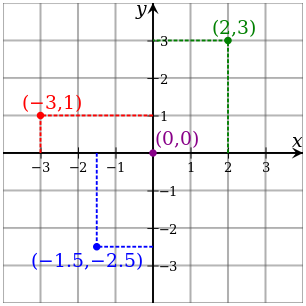
\includegraphics[width=1\textwidth]{figures/cau100.PNG}}
	\caption{penentuan garis/titik dalam diagram kartesius}
	\label{cau100}
	\end{figure}

Perhatikan diagram Cartesius pada gambar di atas. Warna ungu (violet) merupakan pusat koordinat yaitu titik (0,0) yang artinya sumbu x dan y bernilai nol. Untuk warna hijau, pada sumbu x bernilai 2 dan sumbu y bernilai 3 maka koordinat dalam bidang cartesius ditulis (2,3). Untuk warna merah, pada sumbu x bernilai  – 3 dan sumbu y bernilai 1 maka koordinat dalam bidang cartesius ditulis (– 3, 1). Sedangkan untuk warna biru, pada sumbu x bernilai  – 3 dan sumbu y bernilai 1 maka koordinat dalam bidang cartesius ditulis (–1.5 , –2.5).

Menurut wikipedia, istilah Cartesius digunakan untuk mengenang ahli matematika sekaligus filsuf dari Perancis bernama Descartes. Beliau memiliki peranan yang sangat besar dalam menggabungkan aljabar dan geometri (Cartesius adalah latinisasi untuk Descartes). Hasil kerjanya sangat berpengaruh dalam perkembangan geometri analitik, kalkulus, dan kartografi.


